\documentclass[aspectratio=169,pdf,c,xcolor=table]{beamer}
\mode<presentation>{}
\usecolortheme{sag}
\useoutertheme{sag}
\usefonttheme{serif} % default family is serif
\usepackage{LaTeX_macros_bib/macros}
% \RequirePackage[ruled, vlined]{algorithm2e}
\usetikzlibrary{automata,positioning}
\usepackage{pgfplotstable}
\usepackage{csvsimple}
\usetikzlibrary{pgfplots.statistics}
\pgfplotsset{compat=1.16}
% \usepackage{lmodern}% http://ctan.org/pkg/lm
% \usepackage{colortbl}
% \usepackage{environ}
% \usepackage{adjustbox}
\usepackage[font=scriptsize,justification=centering]{caption}
\usepackage{multimedia}
\usepackage{float}
\usepackage{subfig}
\usepackage{caption}
% \usepackage{xmpmulti}
% \usepackage{ragged2e}
\usepackage[authoryear]{natbib}
\let\oldcite=\citep
\renewcommand{\cite}[1]{\textcolor{gray}{\oldcite{#1}}}

\renewcommand{\figurename}{}
\newcommand{\comment}[1]{}
\graphicspath{{./graphics/}}

\renewcommand{\thealgocf}{}
% \captionsetup[algorithm]{labelformat=empty}
% \DeclareCaptionFormat{myformat}{#3}

\newcommand{\secimage}[2]{ \begin{figure}[h] \includegraphics[width=0.8\textwidth,height=0.6\textheight,keepaspectratio]{#1}\caption{\tiny \color{mDarkTeal}{#2}} \end{figure}}
\newcommand{\seccontent}{}
\newcommand{\secinclude}[2]{\renewcommand{\seccontent}{\centering\secimage{#1}{#2}}}

\title[{\textsc{Short Title}}]{\textsc{Long Title for Presentation}}
\author[Author, University]{Author}
\institute[University]{}
\newcommand{\starttcframe}[1][0.5]{\begin{columns}[T]\begin{column}{#1\textwidth}}
\newcommand{\starttcframec}[1][0.5]{\begin{columns}[c]\begin{column}{#1\textwidth}}
\newcommand{\midtcframe}[1][0.5]{\end{column}\begin{column}{#1\textwidth}}
\newcommand{\stoptcframe}{\end{column}\end{columns}}

\newenvironment{tcFrame}[2][0.5]
{\begin{frame}{#2}\starttcframe[#1]}
{\stoptcframe\end{frame}}

\newenvironment{tcFrameC}[2][0.5]
{\begin{frame}{#2}\starttcframec[#1]}
{\stoptcframe\end{frame}}

\setbeamerfont{date}{size=\small}

\newboolean{sectiontoc}
\setboolean{sectiontoc}{true} % default to true

\makeatletter\let\frametextheight\beamer@frametextheight\makeatother
\setbeamercolor{background canvas}{bg=mLightGray}
\setbeamercolor{author}{fg=mDarkTeal, bg=}
\setbeamercolor{institute}{fg=mDarkTeal, bg=}
\setbeamercolor{date}{fg=mDarkTeal, bg=}
\begin{document}

% \AtBeginSection[]
% {
% 	\ifthenelse{\boolean{sectiontoc}}{
% 		\begin{frame}[c]{Outline}
% 			\setbeamertemplate{background canvas}{bg=mLightGray}{}
% 			\setbeamertemplate{section in toc}[sections numbered]
% 			\begin{columns}[c]
% 				\begin{column}{0.5\textwidth}
% 					\vspace{-1cm}
% 					\setbeamercolor{normal text}{bg=mDarkTeal, fg=black!2 }
% 					\setbeamercolor{section in toc}{fg=mDarkRed}
% 					\setbeamercolor{subsection in toc}{fg=black!40!mLightGray}
% 					\tableofcontents[currentsection, sectionstyle=show/shaded, subsectionstyle=show/show/hide]
% 				\end{column}
% 				\begin{column}{0.5\textwidth}
% 					\seccontent
% 				\end{column}
% 			\end{columns}
% 		\end{frame}
% 	}
% }
\newcommand{\toclesssection}[1]{
  \setboolean{sectiontoc}{false}
  \section*{#1}
  \setboolean{sectiontoc}{true}
}
\date{}
%%%%%%%%%%%%%%%%%%%%%%%%%
\begin{frame}[plain]{}
	\centering
	\titlepage
	\vspace{-3em}
	
\includegraphics[width=0.2\textwidth]{graphics/clock.pdf}\\
	{\scriptsize Department of Computer Science\\[-1ex]University of XYZ}
\end{frame}

%%%%%%%%%%%%%%%%%%%%%%%%%
\toclesssection{Coverage using Robots}
%%%%%%%%%%%%%%%%%%%%%%%%%
\subsection{Introduction}

\begin{tcFrame}[0.5]{Coverage using Robots}
	\vspace{5em}
	\centering
	\Large How should robots traverse an environment to efficiently and safely collect data?
	\midtcframe[0.5]
	\centering
	\begin{figure}
		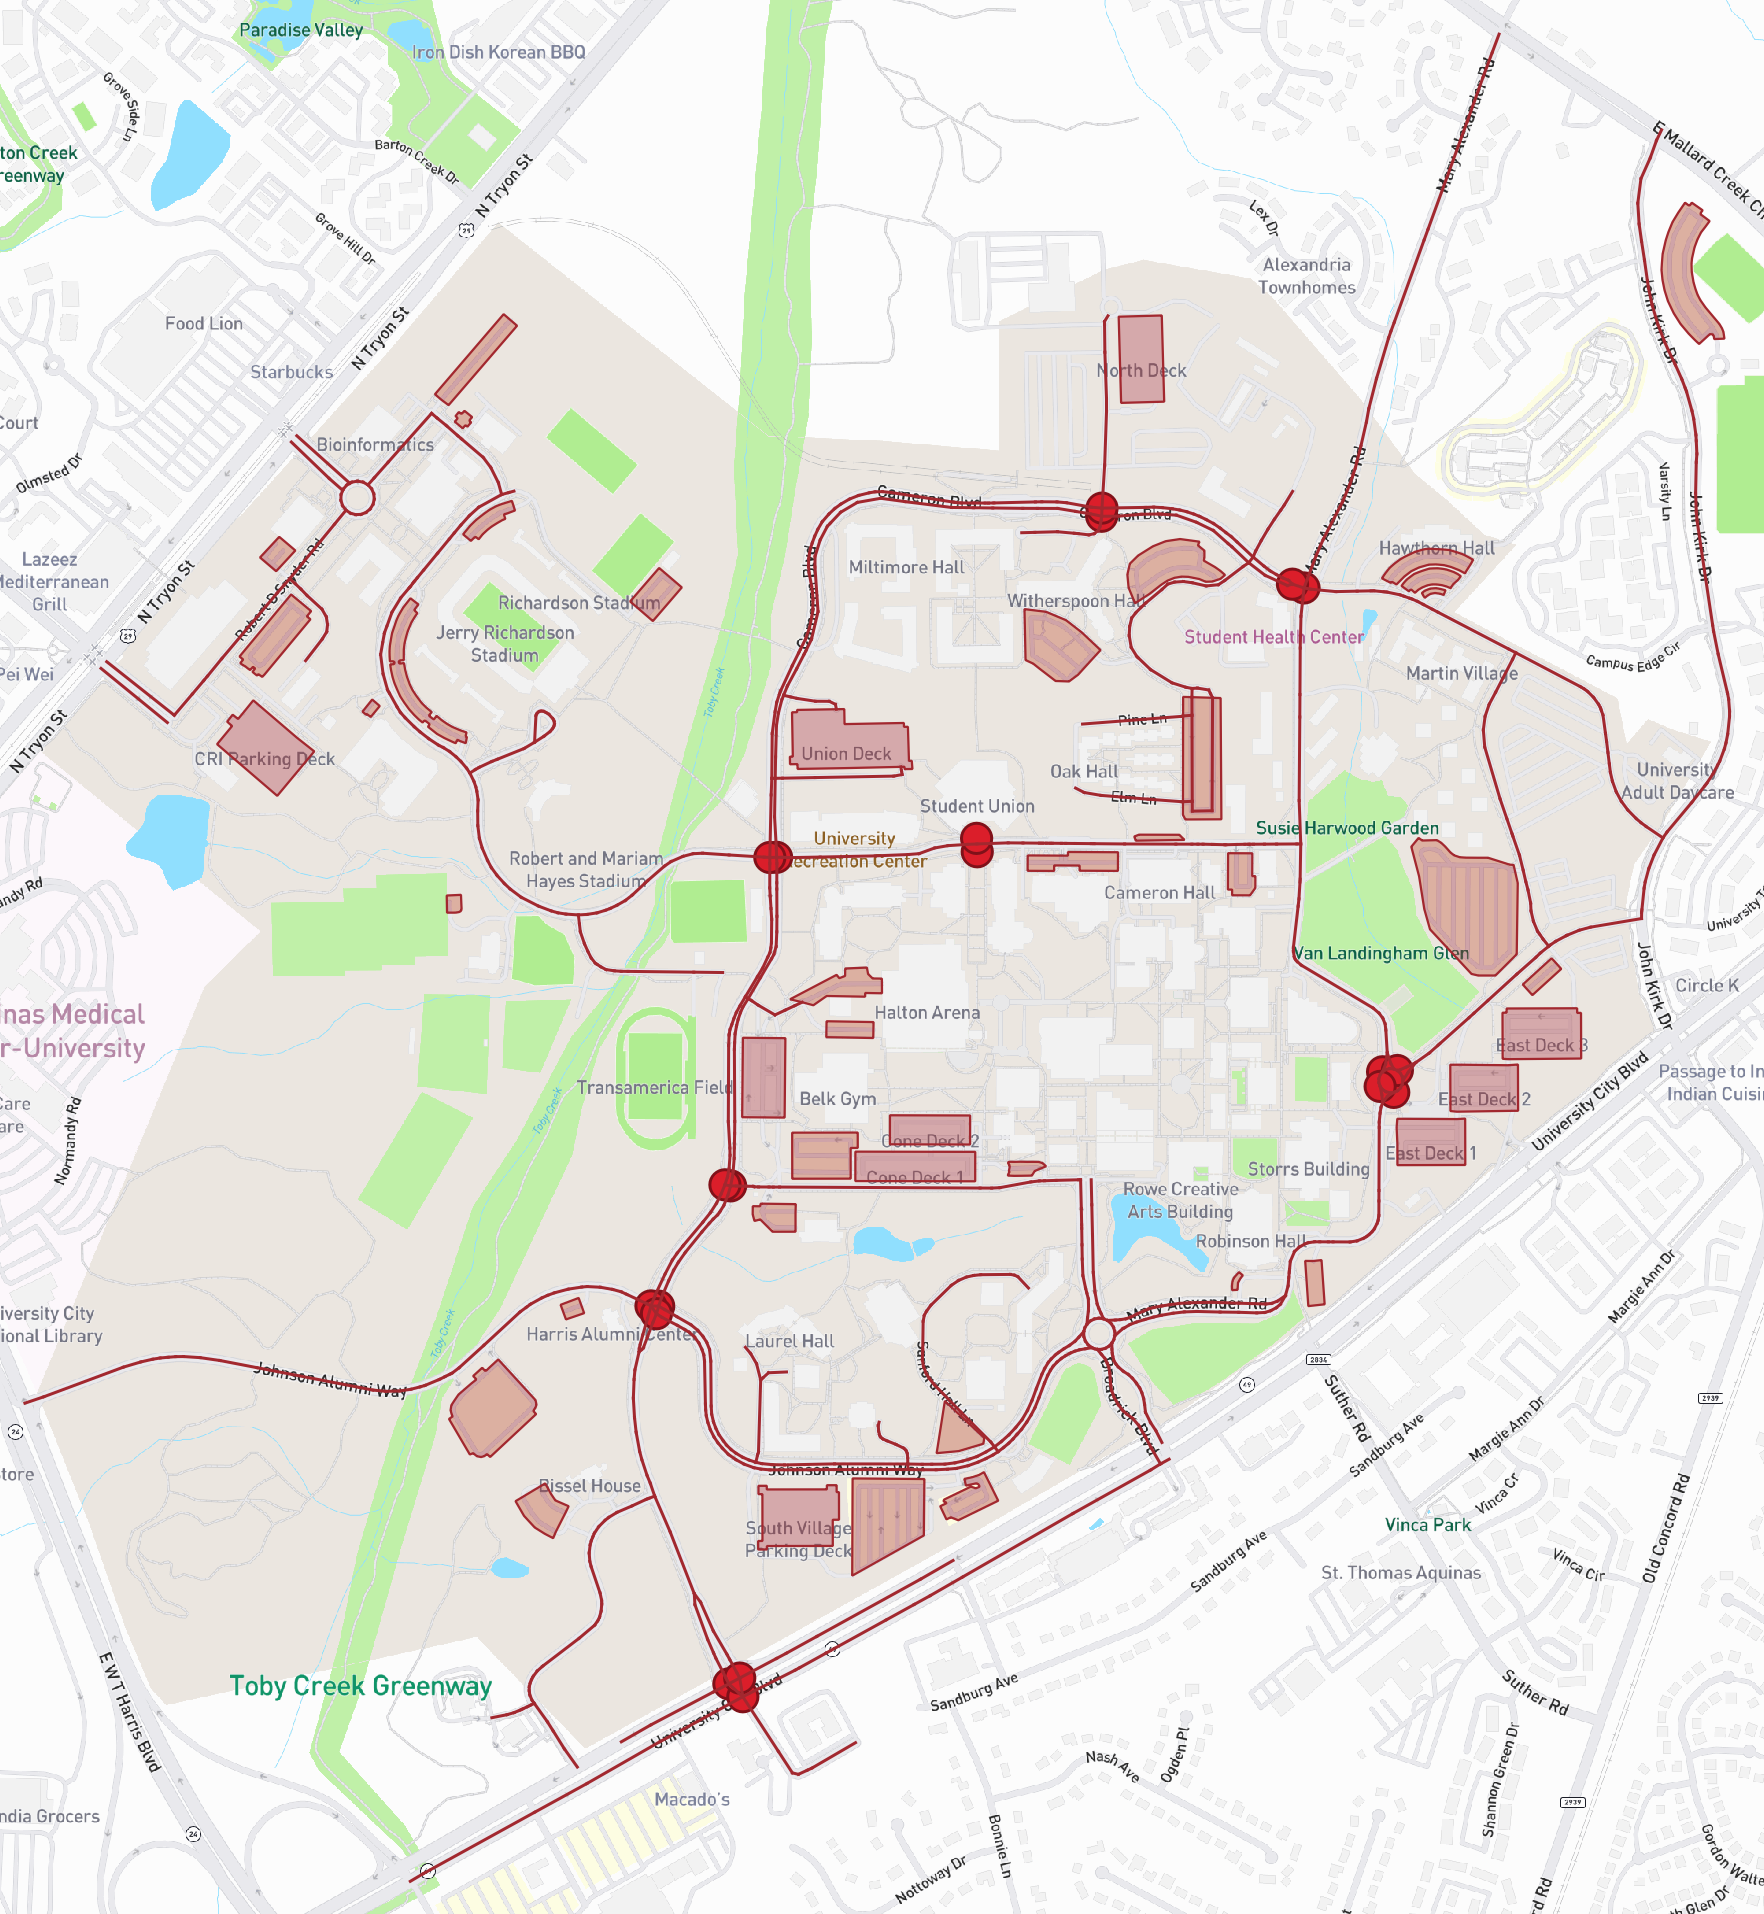
\includegraphics[width=0.7\textwidth]{uncc_gc_map.png}
		\caption{UNC Charlotte Campus}
	\end{figure}
\end{tcFrame}


%%%%%%%%%%%%%%%%%%%%%%%%%

\section*{Outline}
\begin{frame}{Table of Contents}
	\setbeamertemplate{section in toc}[sections numbered]
	\tableofcontents[hideallsubsections]
\end{frame}

\secinclude{konig.png}{{\em Seven bridges of K{\"o}nigsberg}\\ L. Euler. Solutio Problematis ad Geometriam Situs Pertinentis, 1941}
\section{Content}

\begin{frame}[c]
	\vspace{3em}
	\centering
	Thank You!
\end{frame}

%%%%%%%%%%%%%%%%%%%%%%%%%

\section*{References}
\bibliographystyle{abbrvnat}
\bibliography{LaTeX_macros_bib/references}

\end{document}

